% For LaTeX-Box: root = stat305-pexam1.Rnw
\documentclass[addpoints]{examsetup}

\usepackage{etoolbox}
\usepackage{tikz,pgfplots}

\makeatletter
\def\maxwidth{ %
  \ifdim\Gin@nat@width>\linewidth
    \linewidth
  \else
    \Gin@nat@width
  \fi
}
\makeatother
\usepackage{pdfpages} 
\definecolor{fgcolor}{rgb}{0.345, 0.345, 0.345}
\newcommand{\hlnum}[1]{\textcolor[rgb]{0.686,0.059,0.569}{#1}}%
\newcommand{\hlstr}[1]{\textcolor[rgb]{0.192,0.494,0.8}{#1}}%
\newcommand{\hlcom}[1]{\textcolor[rgb]{0.678,0.584,0.686}{\textit{#1}}}%
\newcommand{\hlopt}[1]{\textcolor[rgb]{0,0,0}{#1}}%
\newcommand{\hlstd}[1]{\textcolor[rgb]{0.345,0.345,0.345}{#1}}%
\newcommand{\hlkwa}[1]{\textcolor[rgb]{0.161,0.373,0.58}{\textbf{#1}}}%
\newcommand{\hlkwb}[1]{\textcolor[rgb]{0.69,0.353,0.396}{#1}}%
\newcommand{\hlkwc}[1]{\textcolor[rgb]{0.333,0.667,0.333}{#1}}%
\newcommand{\hlkwd}[1]{\textcolor[rgb]{0.737,0.353,0.396}{\textbf{#1}}}%
\let\hlipl\hlkwb

\usepackage{ulem}

\usepackage{framed}
\makeatletter
\newenvironment{kframe}{%
 \def\at@end@of@kframe{}%
 \ifinner\ifhmode%
  \def\at@end@of@kframe{\end{minipage}}%
  \begin{minipage}{\columnwidth}%
 \fi\fi%
 \def\FrameCommand##1{\hskip\@totalleftmargin \hskip-\fboxsep
 \colorbox{shadecolor}{##1}\hskip-\fboxsep
     % There is no \\@totalrightmargin, so:
     \hskip-\linewidth \hskip-\@totalleftmargin \hskip\columnwidth}%
 \MakeFramed {\advance\hsize-\width
   \@totalleftmargin\z@ \linewidth\hsize
   \@setminipage}}%
 {\par\unskip\endMakeFramed%
 \at@end@of@kframe}
\makeatother

\definecolor{shadecolor}{rgb}{.97, .97, .97}
\definecolor{messagecolor}{rgb}{0, 0, 0}
\definecolor{warningcolor}{rgb}{1, 0, 1}
\definecolor{errorcolor}{rgb}{1, 0, 0}
\newenvironment{knitrout}{}{} % an empty environment to be redefined in TeX

\usepackage{alltt}
\usepackage{graphicx, fancyhdr}
\usepackage{amsmath, amsfonts}
\usepackage{color}
\usepackage{hyperref}

\newcommand{\blue}[1]{{\color{blue} #1}}

\setlength{\topmargin}{-.5 in} 
\setlength{\textheight}{9 in}
\setlength{\textwidth}{6.5 in} 
\setlength{\evensidemargin}{0 in}
\setlength{\oddsidemargin}{0 in} 
\setlength{\parindent}{0 in}
\newcommand{\ben}{\begin{enumerate}}
\newcommand{\een}{\end{enumerate}}



%% For LaTeX-Box: root = stat105_exam1_info.tex 
%%%%%%%%%%%%%%%%%%%%%%%%%%%%%%%%%%%%%%%%%%%%%%%%%%%%%%%%%%%%%%%%%%%%%%%%%%%%%%%%
%  File Name: stat105_exam1_info.tex
%  Purpose:
%
%  Creation Date: 24-09-2015
%  Last Modified: Thu Sep 24 13:51:36 2015
%  Created By:
%%%%%%%%%%%%%%%%%%%%%%%%%%%%%%%%%%%%%%%%%%%%%%%%%%%%%%%%%%%%%%%%%%%%%%%%%%%%%%%%
\newcommand{\course}[1]{\ifstrempty{#1}{STAT 105}{STAT 105, Section #1}}
\newcommand{\sectionNumber}{B}
\newcommand{\examDate}{October 1, 2015}
\newcommand{\semester}{FALL 2015}
\newcommand{\examNumber}{II}

\newcommand{\examTitle}{Exam \examNumber}

\runningheader{\course{\sectionNumber}}{Exam \examNumber}{\examDate}
\runningfooter{}{}{Page \thepage of \numpages}

\newcommand{\examCoverPage}{
   \begin{coverpages}
   \centering
   {\bfseries\scshape\Huge Exam I \par}
   \vspace{1cm}
   {\bfseries\scshape\LARGE \course{\sectionNumber} \par}
   {\bfseries\scshape\LARGE \semester \par}

   \vspace{2cm}

   \fbox{\fbox{\parbox{5.5in}{\centering 

      \vspace{.25cm} 
      
      {\bfseries\Large Instructions} \\

      \vspace{.5cm} 

      \begin{itemize}
         \item  The exam is scheduled for 80 minutes, from 8:00 to 9:20 AM. At 9:20 AM the exam will end.\\
         \item  A forumula sheet is attached to the end of the exam. Feel free to tear it off.\\
         \item  You may use a calculator during this exam.\\
         \item  Answer the questions in the space provided. If you run out of room, continue on the back of the page. \\
         \item  If you have any questions about, or need clarification on the meaning of an item on this exam, please ask your instructor. No other form of external help is permitted attempting to receive help or provide help to others will be considered cheating.\\
         \item  {\bfseries Do not cheat on this exam.} Academic integrity demands an honest and fair testing environment. Cheating will not be tolerated and will result in an immediate score of 0 on the exam and an incident report will be submitted to the dean's office.\\
      \end{itemize}

   }}}

   \vspace{2cm}

   \makebox[0.6\textwidth]{Name:\enspace\hrulefill}

   \vspace{1cm}

   \makebox[0.6\textwidth]{Student ID:\enspace\hrulefill}
   \end{coverpages}

}


\newcommand{\course}[1]{\ifstrempty{#1}{STAT 305}{STAT 305, Section #1}}
\newcommand{\sectionNumber}{3}
\newcommand{\examDate}{October 17, 2019}
\newcommand{\semester}{FALL 2019}
\newcommand{\examNumber}{II}

\usepackage{Sweave}
\begin{document}
\Sconcordance{concordance:stat305-pq2.tex:stat305-pq2.Rnw:%
1 81 1 1 0 3 1 1 9 7 1 1 31 11 1 1 3 1 2 94 1}


%-- : R code (Code in Document)


\examCoverPage

\begin{questions}

\question \textbf{Champions Red Wine}
%-- : R code (Code in Document)

Oenophiles, or connoisseurs of fine wines, have been benefitted by sort of open information sharing we have in the days of online auctions. 
By monitoring the prices for which sought after bottles actually sell for, wine enthusiasts are able to both determine whether or not they are getting a fair price and whether or not they might make a nice profit by selling off a few of the bottles they have in storage.
Before this era of easy and free data though, there was one source of information that stood above all the others: \textit{Le Champions de vin rouge}, a guide to the world of fine wines published in 1997.
While the information contained it in is largely still relevant in general, the price index has become somewhat outdated.

Or has it? 
Is it possible that the prices from the guide in 1997 could help us understand the market today?
A certain statistician decided to do a deep analysis of the relationship between the cost of wine bottles in the 1997 book and the actual prices the same bottles fetched on open auction sites recently. 
The dataset he created consists of the last 500 bottles with publically available auction prices that were also listed in \textit{Le Champions de vin rouge} price index.

\begin{center}
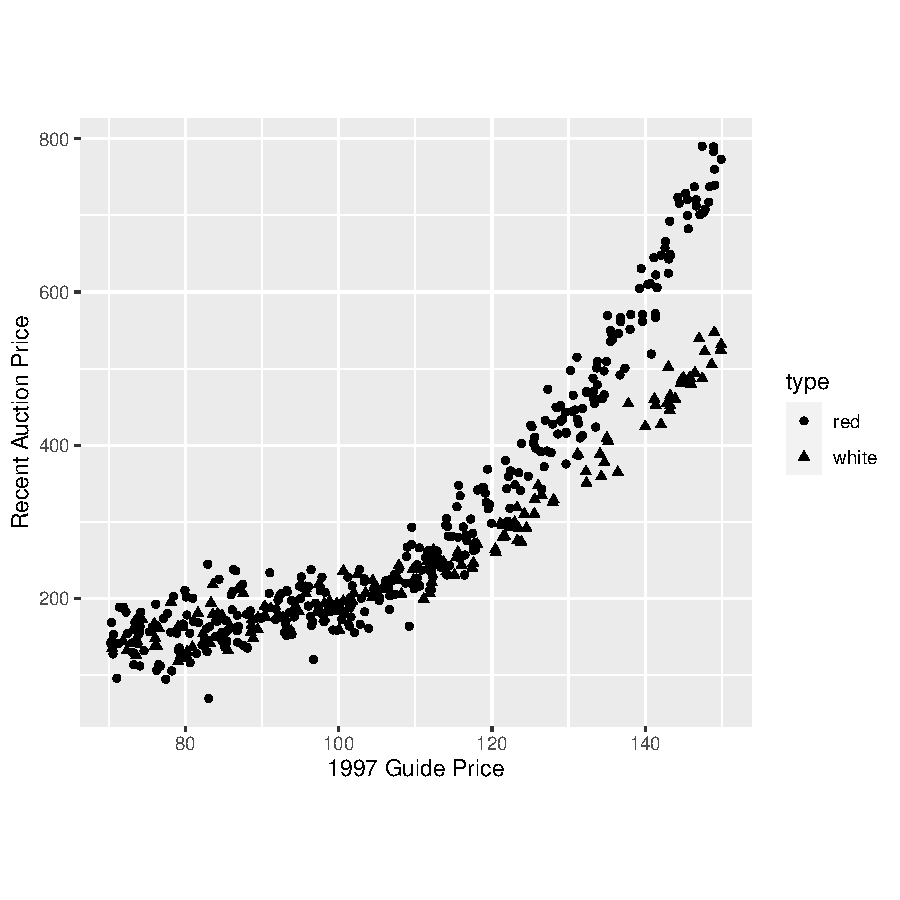
\includegraphics{stat305-pq2-003}
\end{center}
\pagebreak
Here are some summaries of the dataset with the 1997 Guide Price as $x$ and the Recent Auction Price as $y$.

$$
\sum_{i=1}^{500} x_i = 54348 \hspace{3cm} \sum_{i=1}^{500} x_i^2 = 6164828 \\
$$

$$
\sum_{i=1}^{500} y_i = 146782 \hspace{3cm} \sum_{i=1}^{500} y_i^2 = 55928348 \\
$$

$$
\sum_{i=1}^{500} x_i y_i = 17573001
$$

\begin{parts}
   \part Using the summaries, fit a linear relationship between \textbf{1997 Guide Price} (x) and \textbf{Recent Auction Price} (y). 
   \begin{subparts}
      \subpart[5] Write the equation of the fitted linear relationship. 
      \vspace{4cm}
      \subpart[5] Find and interpret the value of $R^2$ for the fitted linear relationship.
      \vspace{3cm}
      \subpart[5] Using the fitted line, provide a predicted Recent Auction Price when the 1997 Guide Price was \$120.
      \vspace{3cm}

   \end{subparts}


   \part 
   The JMP output below comes from fitting a quadratic model using $x$ and $x^2$ for \textit{Red Wine Only} (left) and \textit{White Wine Only} (right).



      \begin{figure}
  \begin{minipage}[b]{.5\linewidth}
     \centering
    		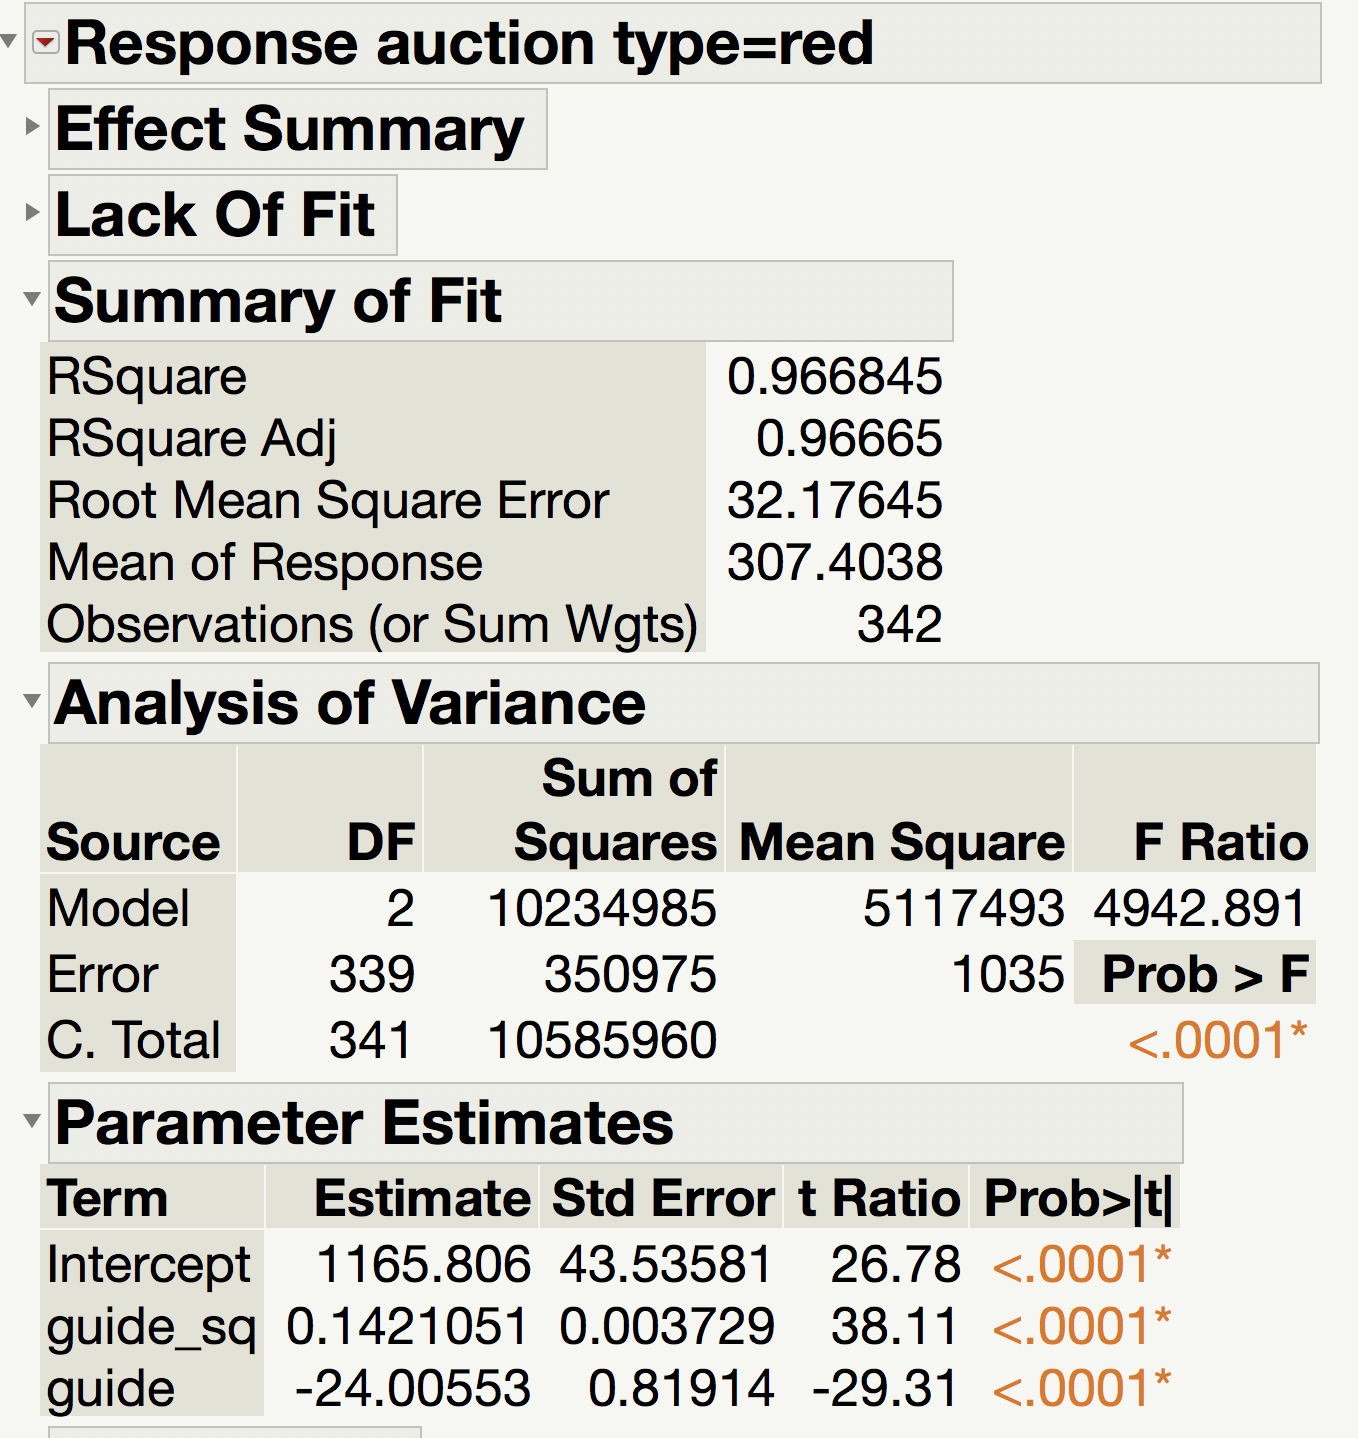
\includegraphics[scale=.2]{figure/red-wine-quadratic.png}
     \subcaption{Red wine}
  \end{minipage}%
  \begin{minipage}[b]{.5\linewidth}
     \centering\
    	  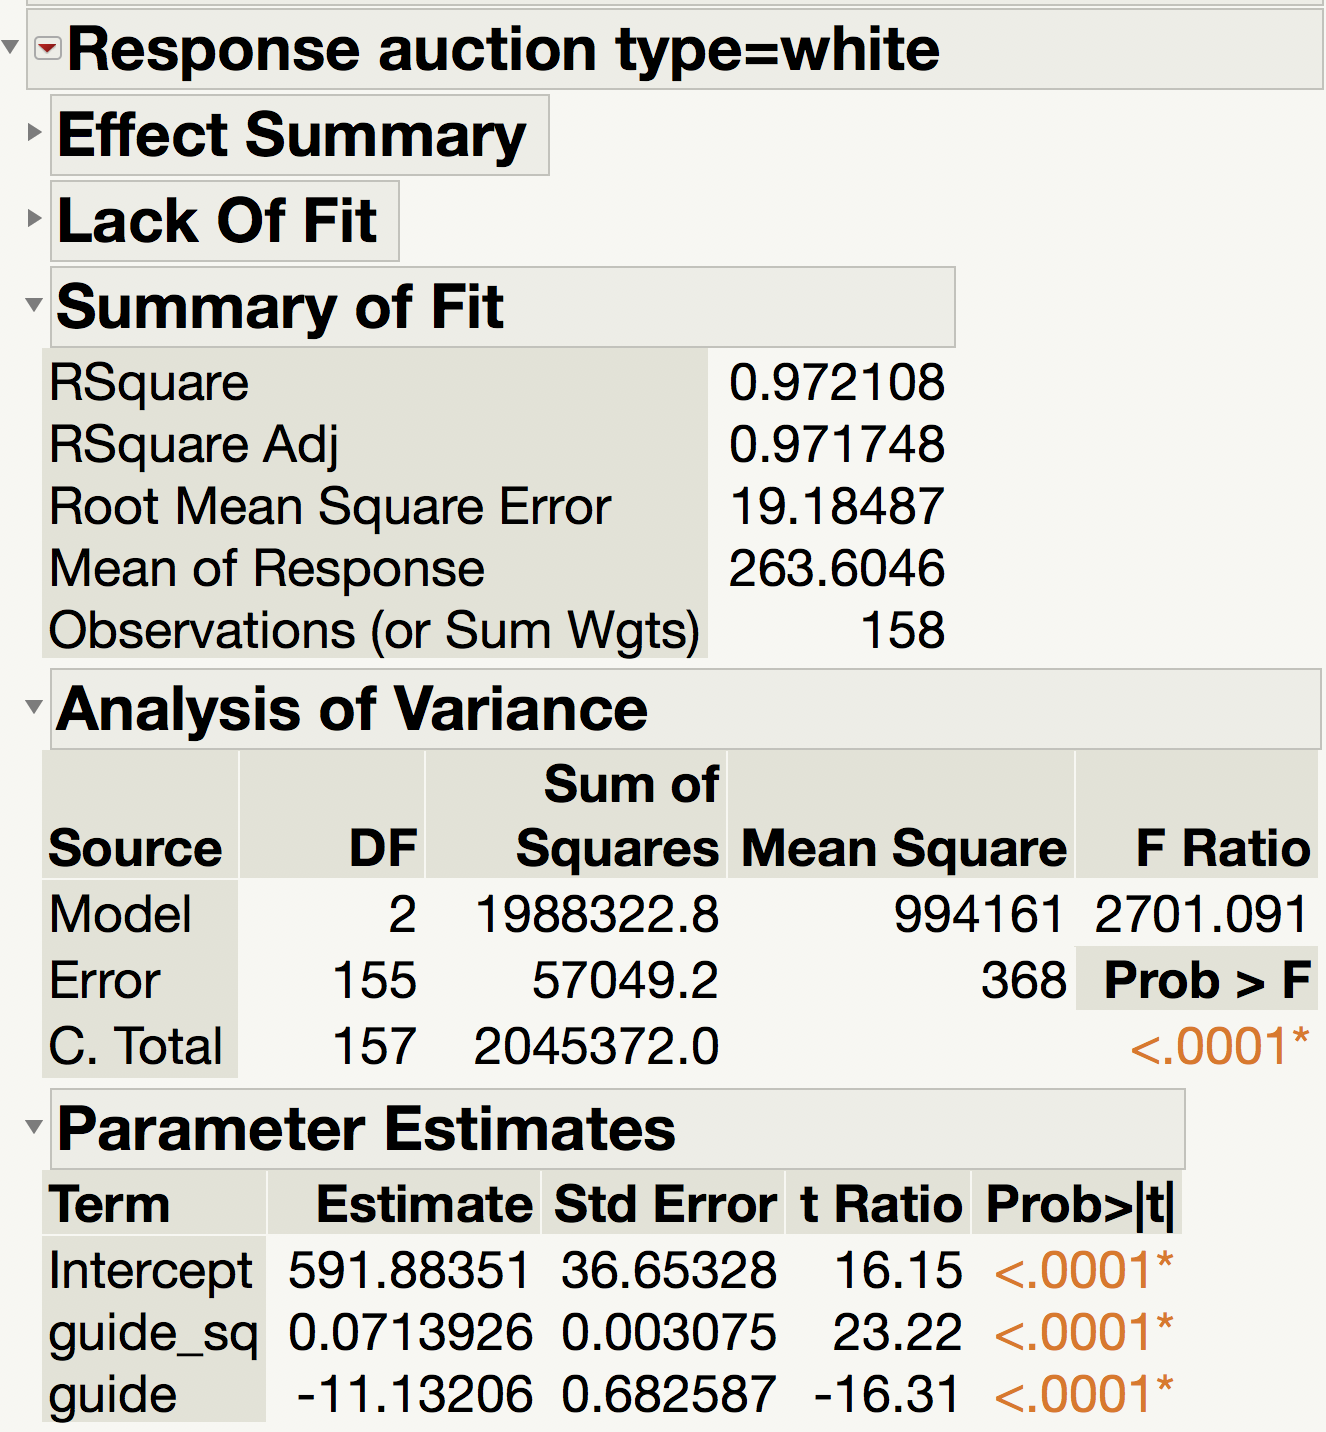
\includegraphics[scale=.2]{figure/white-wine-quadratic.png}
     \subcaption{White wine}
  \end{minipage}
  \caption{JMP output of fitting a quadratic model using $x$ and $x^2$ for \textit{Red Wine Only} (left) and \textit{White Wine Only} (right). }
\end{figure}




   \begin{subparts}
      \subpart[5] Write the equation of the fitted quadratic relationship \textit{for Red Wines} i.e the polynomial to degree two. 
      \vspace{2cm}
      \subpart[5] Write the equation of the fitted quadratic relationship \textit{for White Wines}  i.e the polynomial to degree two. . 
      \vspace{2cm}
      \subpart[5] Interpret the value of $R^2$ for the two fitted quadratic relationships.
      \vspace{2cm}
      \subpart[5] Using the fitted quadratic relationship, provide a predicted value of Recent Auction Price for a red wine with 1997 Guide Price of \$120.(note that, in this question, it is also possible if you get a negative number for the auction price)
      \vspace[4cm]
   \end{subparts}
\end{parts}
\pagebreak
\question
      Suppose $X$ is a discrete random variable with following probability function:

      $$f(x) = \begin{cases} 0.1 & x = -2, 0, 2 \\\\ 0.35 & x = -1, 1 \\\\ 0 & o.w. \end{cases}$$
      
      \begin{subparts}
            \subpart[2] Find $P(X = 0)$ \vspace{2.5cm}
            \subpart[2] Find $P(X \le 0)$ \vspace{2.5cm}
            \subpart[2] Find $P(\vert{X}\vert > 1)$ \vspace{2.5cm}
            \subpart[3] Find the CDF of $X$.\vspace{2.5cm}
            \subpart[3] Find the expected value of $X$.\vspace{2.5cm}
            \subpart[3] Find the variance of $X$.\vspace{2.5cm}
      \end{subparts}
\pagebreak      
% \question
% Suppose a standup comedian plans to give a total of $n= 5$ jokes in an entire 2-hour performance. Call a joke a succes if at least one audience member laughs. If no audience member laughs, the joke is a failure. Assume that all the jokes are equally funny, with $p= p(success)= 0.2$. Let $X$ be the random variable that denotes the number of jokes out of the total 5 were successes. 
% \begin{subparts}
%       \subpart[3] Precisely state the distribution of $X$, giving the values of any parameters necessary.\vspace{2cm}
%       \subpart[3] Calculate the probability that the whole night is a failure: i.e., $P(no\ laughs)$\vspace{3cm}
%       
%       \subpart[3] Caculate the probability that the comedian tells at least 4 successful jokes.\vspace{3cm}
%       
%       \subpart[3] Calculate the expected number of successfull jokes. \vspace{2cm}
%       
%       \subpart[3] Calculate the standard deviation of $X$\vspace{2cm}
% 
% 
% \end{subparts}
% \pagebreak

\end{questions}
\end{document}
